\documentclass[serif,9pt,xcolor=dvipsnames]{beamer}
\usetheme{default}

%\usepackage[english]{babel}    % deutsche Sonderzeichen, Trennmuster, etc
\usepackage[german]{babel}    % deutsche Sonderzeichen, Trennmuster, etc

\usepackage[T1]{fontenc} 
\usepackage[utf8]{inputenc}  % deutsche Umlaute


\usetheme[]{Warsaw}
%\usetheme[]{Rochester}

%  \usecolortheme[named=Brown]{structure} 
%\usecolortheme[]{crane} 
%\usecolortheme[]{rose} 
\usecolortheme[]{christian1} 

% Mathekram
%\usepackage{amsmath}
%\usepackage{amsfonts}
%\usepackage{amssymb}

% Graphiken
%\usepackage{epsfig}            % Paket zum Einbinden von postscript Graphiken
\usepackage{graphicx}		% Andere Graphikdateien einbinden
\usepackage{float}             % Hilfesmakros beim Positionieren von Graphiken
\usepackage{color}
%\usepackage{subfig}
\usepackage{textcomp}

\usepackage[sc]{mathpazo}	%FONT

\usepackage{relsize} % Notwenfig für verbatim
\usepackage{listings}
\usepackage{verbatim}


%% GLEGRAPHICS
\graphicspath{{./bilder/gleplots/}}

\newcommand{\includeglegraphics}[1]{  
%\includegraphics[]{#1.pdf}
\input{#1.inc}   
}

% \newcommand{\listing}[1]{
%    {\small 
%   \begin{lstlisting}
%    
%   \end{lstlisting}}
% }

\newcommand{\Th}{\vartheta}

%\newcommand{\Th}{\vartheta}


\definecolor{feedforwardpath}{rgb}{0.0,1,0.0}
\definecolor{feedbackpath}{rgb}{1.0,0.0,0.0}

\DeclareRobustCommand{\vec}[1]{{\mbox{\mathversion{bold}\ensuremath{#1}}}}
\DeclareRobustCommand{\mat}[1]{{\mbox{\mathversion{bold}\ensuremath{#1}}}}

\title[]{OpenRTDynamics --- A framework for the implementation of real-time controllers}
	\subtitle{} %Mehrgrößenregelung einer Neuro-Prothese zur Generierung von Bewegungen  der oberen Extremität mittels Neuromuskulärer Elektrostimulation (NMES)
\date{May 2014}
\author{Christian Klauer$^{1}$\\
\tiny $^{1}$Control Systems Group, Technische Universität Berlin\\
Kontakt: klauer@control.tu-berlin.de
}




\begin{document}
% \frame[plain]{\titlepage}

% \author{Christian Klauer$^{1}$}



\begin{frame}
  \maketitle
\end{frame}


\begin{frame}

\textbf{OpenRTDynamics contains}

 \begin{itemize}
  \item A simulator/interpreter for discrete-time dynamical systems
  \item A Scilab-toolbox for describing these systems in an block/signal based way.
  \item Many plugins (e.g. state machines, threads (multiple main loops), UDP-communication, remote control via GUIs, ...)
 \end{itemize}

\textbf{Compared to other systems it features}
\begin{itemize}
 \item A new concept of defining schematics that enables well structured and easy maintainable code as projects get bigger.
 \item Nesting schematics of infinite depth: e.g. ability to reset and/or switch between sub-schematics (state machines).
 \item Specially defined parts of the real-time implementation can be exchanged on-line.
% \item Does not require a code compilation step for generating real-time code, because of online interpretation.
% \item On-line exchange of schematics
\end{itemize}


\end{frame}



\begin{frame}

 \frametitle{General Overview}



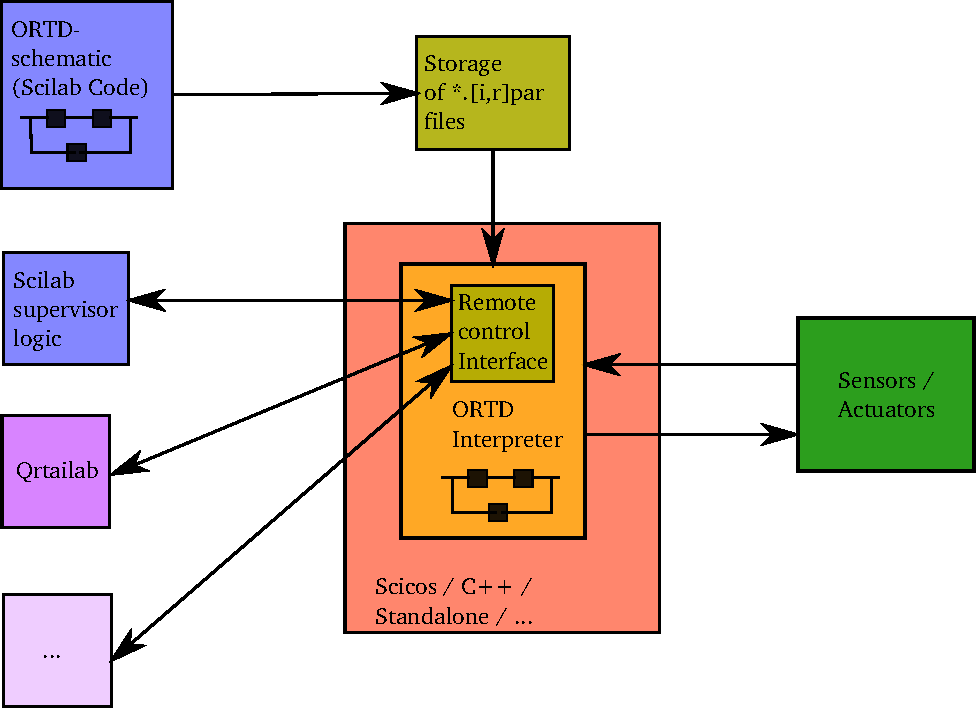
\includegraphics[trim=0mm 0mm 0mm 0mm, clip,width=0.95\linewidth]{../pictures/ortd_principle.pdf}

\end{frame}



\begin{frame}
\frametitle{Targets / Interfaces}

\textbf{Target systems so far:}
\begin{itemize}
 \item Linux incl. realtime preemption
 \item Linux on ARM-based systems (Beaglebone, Raspberry Pi, ...)
 \item Android
 \item Easily portable if an implementation of Posix Threads is available.
\end{itemize}


\textbf{Possible modes of operation}
  \begin{itemize}
   \item Standalone applications using the \texttt{ortd}-command
   \item Embedded into a Scicos-block
   \item API for C++/C projects available { \texttt{libortd.so} }
  \end{itemize}

\end{frame}



\begin{frame}[fragile]
  \frametitle{Interface to Scicos}

  \centering 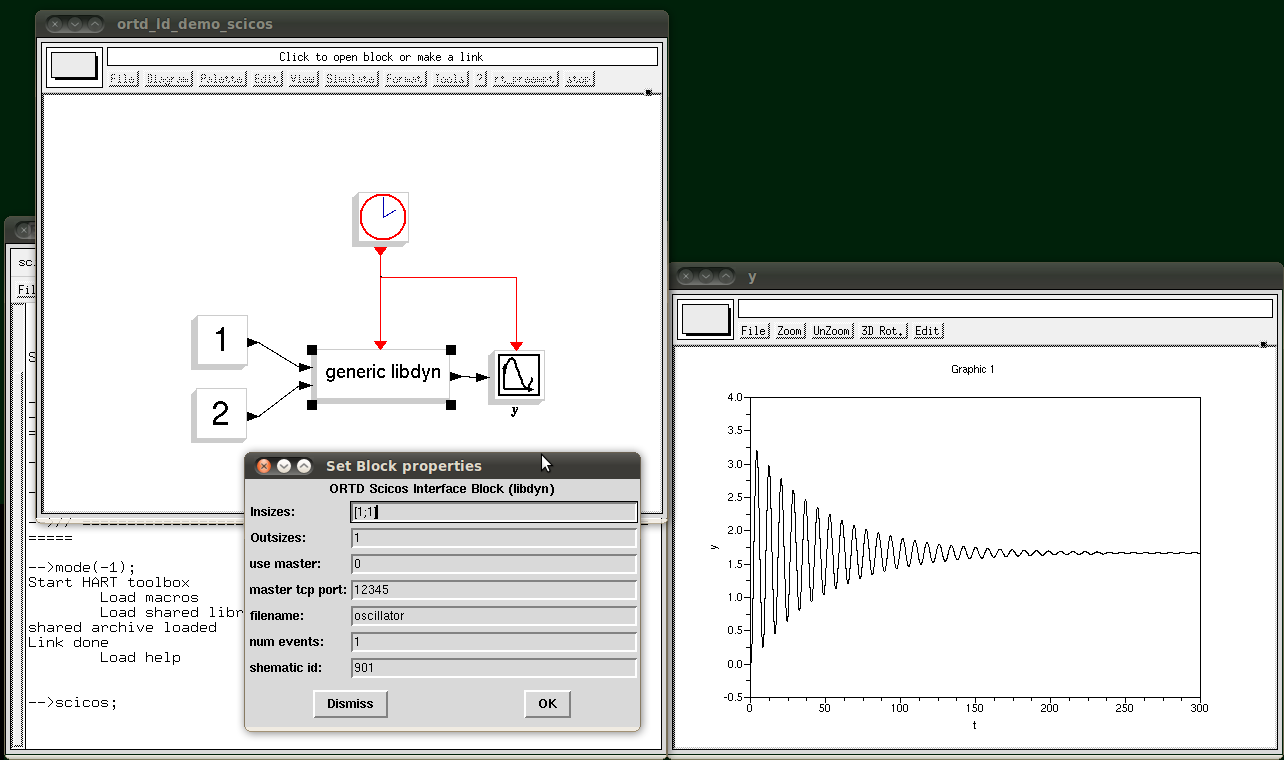
\includegraphics[trim=0mm 0mm 80mm 80mm, clip, width=1\linewidth]{figures/ortd_scicos_interface.png} 

  \begin{itemize}
   \item Specification of the in- and output port sizes along the name of the schematic to load.
   \item Multiple interface blocks within one Scicos diagram are possible
  \end{itemize}

\end{frame}


\begin{frame}[fragile]
  \frametitle{Standalone}

  \centering 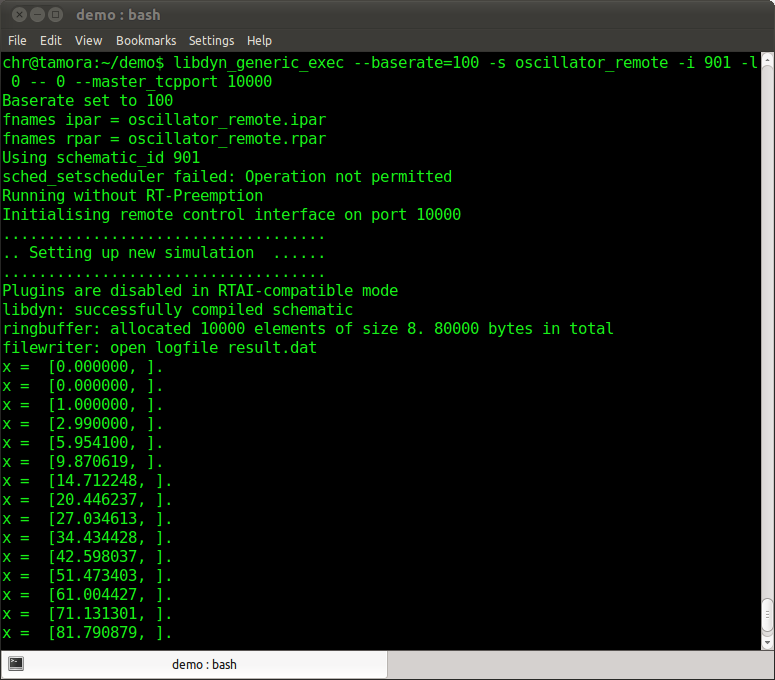
\includegraphics[trim=0mm 0mm 00mm 00mm, clip, width=0.8\linewidth]{figures/start_from_console.png} 

  \begin{itemize}
   \item Simulation mode or real-time execution with RT-Preempt scheduling or using soft RT.
  \end{itemize}

\end{frame}





\begin{frame}[fragile]
    \frametitle{Signals and Blocks in ORTD}

\textbf{How schematics are defined:}

  \begin{itemize}
  \item \textbf{Signals} are represented by a special Scilab variables.
  \item \textbf{Blocks} are defined by calls to special Scilab functions (\texttt{ld\_}-prefix). They may take input signal variables and may return new signal variables.
  \end{itemize}

\textbf{An Example:}
  \begin{itemize}
  \item A linear combination of two signals ( $y=u_1 - u_2$ ) is implemented:
  \end{itemize}

  {\small 
  \begin{lstlisting}
    [sim, y] = ld_add(sim, defaultevents, list(u1, u2), [ 1, -1 ] );
  \end{lstlisting}}
    

  \begin{itemize}
  \item A time-discrete transfer function is implemented like:
  \end{itemize}

  {\small 
  \begin{lstlisting} 
      [sim, y] = ld_ztf(sim, defaultevents, u, (1-0.2)/(z-0.2) );
  \end{lstlisting}}

\textbf{Please Note:}
  \begin{itemize}
  \item For all calculations the toolbox functions must be used. \textbf{Not possible:} \texttt{y = u1 - u2}, whereby \texttt{u1} and \texttt{u2} are signal variables.
  \end{itemize}
  


\end{frame}




\begin{frame}[fragile]
\frametitle{Signals and Blocks in ORTD}
 
 \textbf{Some more explanation:}

{\small 
\begin{lstlisting}
   [sim, y] = ld_add(sim, defaultevents, list(u1, u2), [ 1, -1 ] );
\end{lstlisting}}
 
 \begin{itemize}
   \item The variable \texttt{sim} is technically used to emulate object-orientated behaviour in Scilab.
   \item \texttt{defaultevents} must be zero.
 \end{itemize}

 \vspace{1.5cm}

\textbf{Help:}
 \begin{itemize}
  \item A list of available blocks may be browsed using the Scilab-help functionality, e.g. try \texttt{help ld\_add}.
 \end{itemize}
 

\end{frame}



\begin{frame}[fragile]
  \frametitle{A working example -- part 1}

\textbf{Definition:} Within Scilab by writing a function that describes the blocks and connections:

\centering 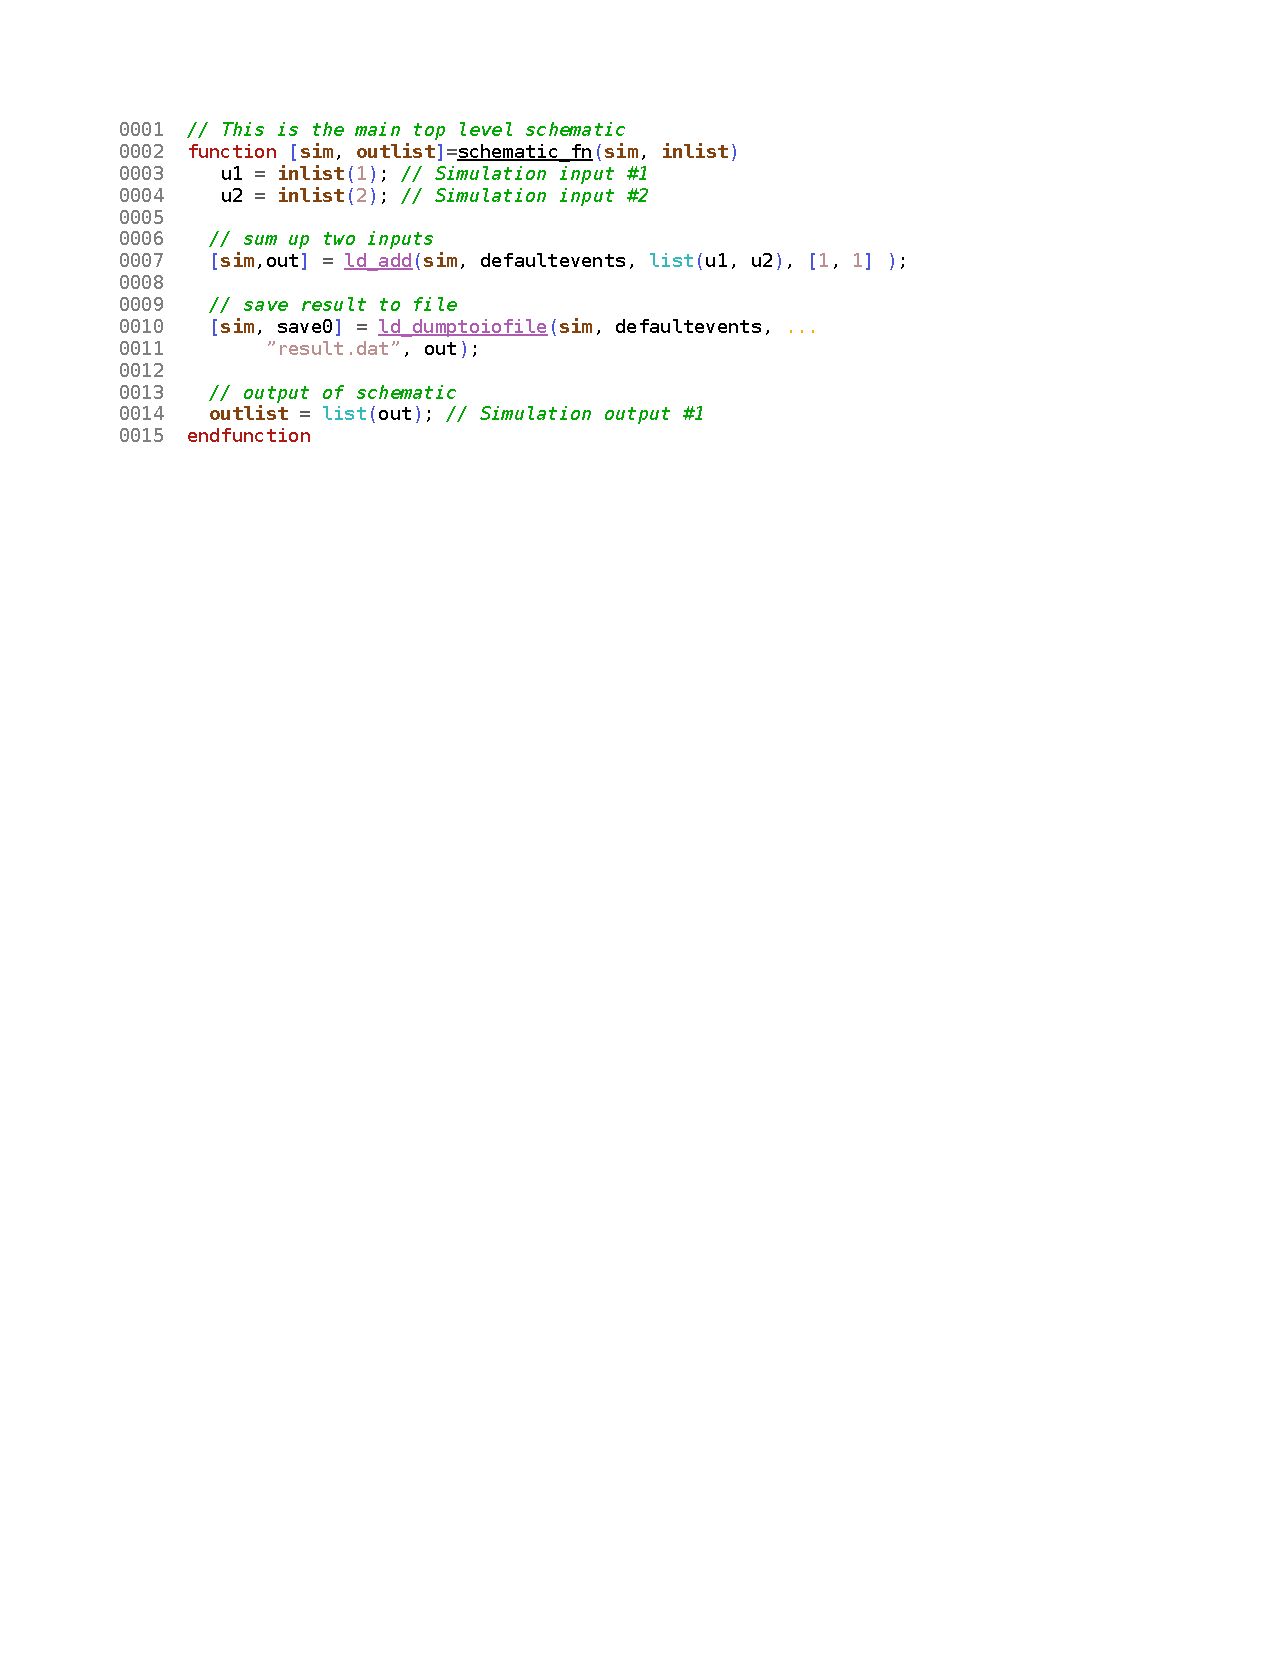
\includegraphics[trim=3cm 20cm 4cm 1.4cm, clip, width=0.85\linewidth]{figures/schematic_fn.pdf} 


% schematic_fn

\begin{itemize}
 \item It takes the simulation object \texttt{sim} as well as a list of in- and  outputs.
\end{itemize}


\end{frame}


\begin{frame}[fragile]
  \frametitle{A working example -- part 2}

% \begin{itemize}
%  \item A schematic is generated via the following code. 
% \end{itemize}

  \textbf{Generation:} A set of function calls trigger evaluation of the functions describing the schematic.


\centering 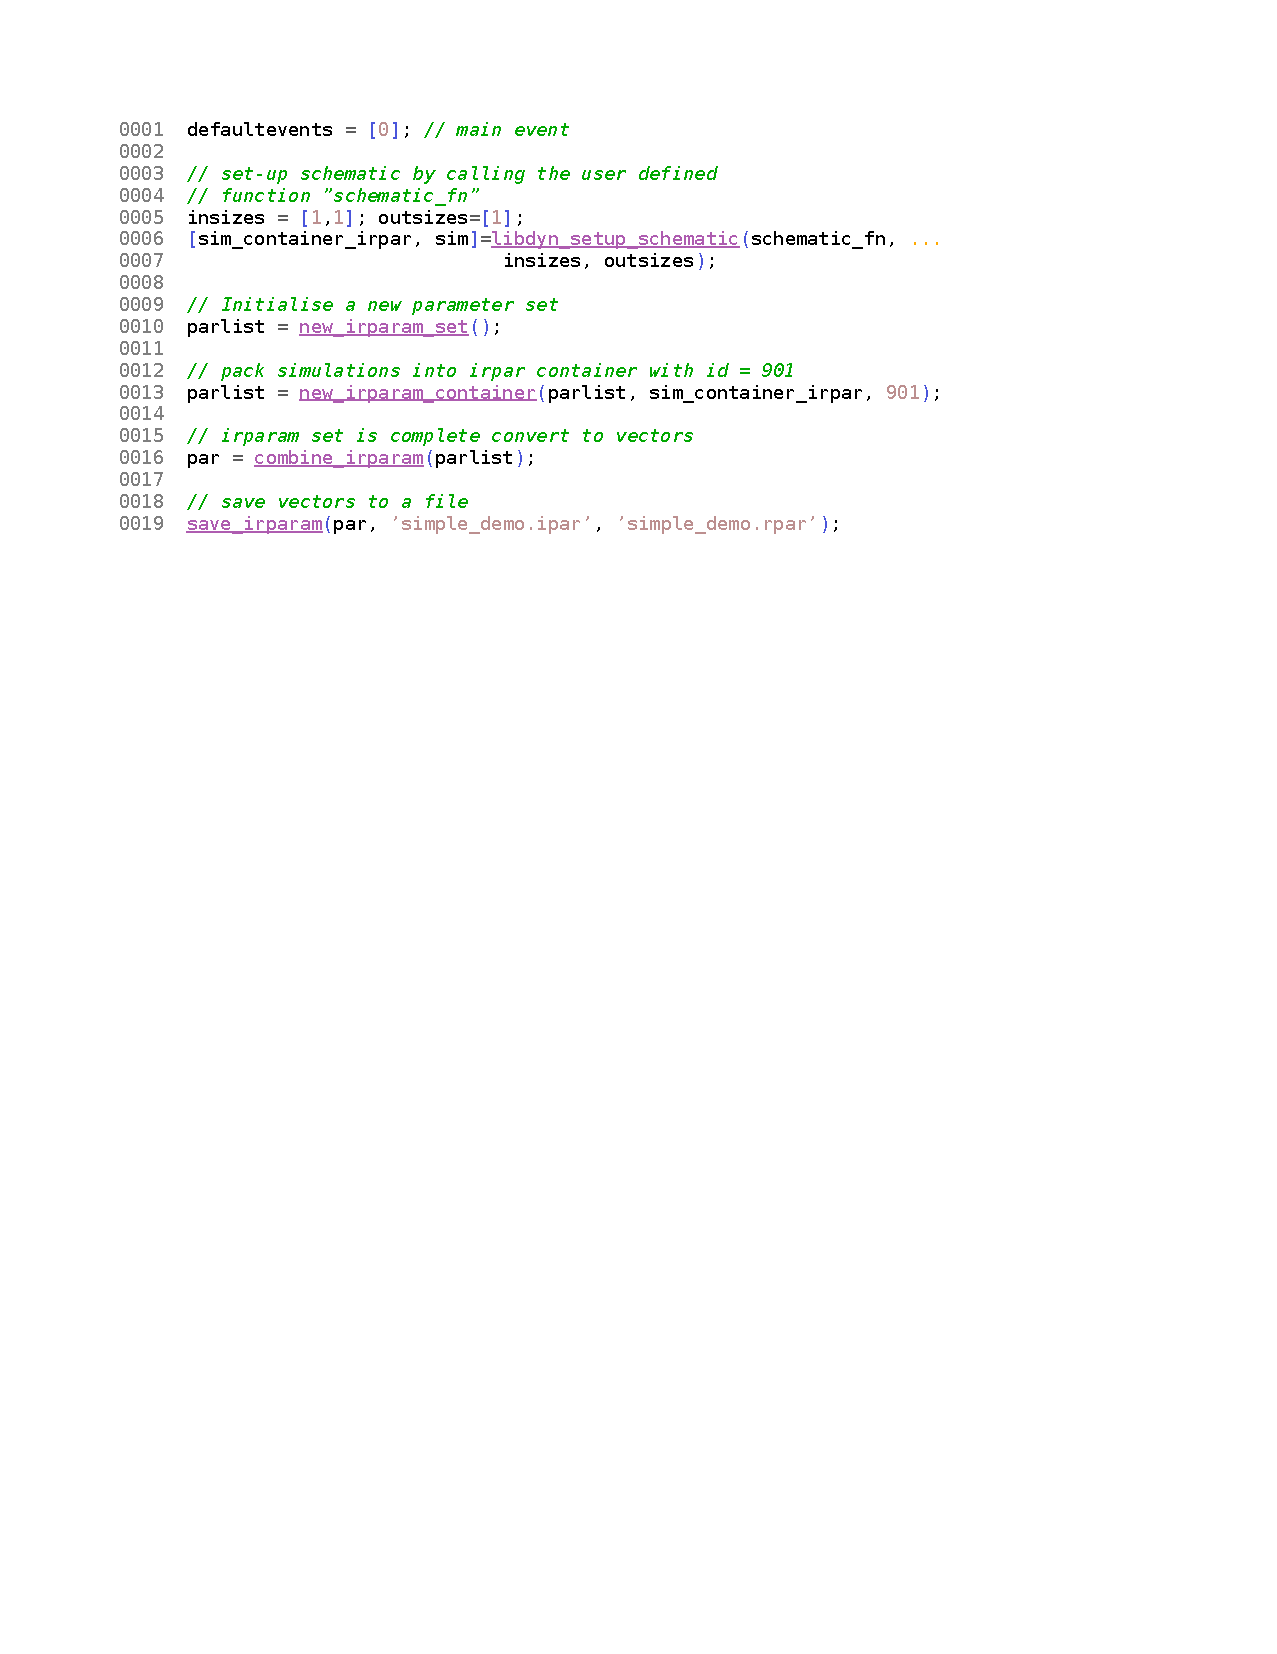
\includegraphics[trim=3cm 19cm 4cm 1.4cm, clip, width=0.85\linewidth]{figures/schematic_fn_load.pdf} 

\begin{itemize}
%  \item The function \texttt{libdyn\_setup\_schematic} calls the function describing the schematic.
 \item The schematic is saved to disk by \texttt{save\_irparam}.
\end{itemize}


% {\small 
% \begin{lstlisting} 
% defaultevents = [0]; // main event
% 
% // set-up schematic by calling the user defined
% // function "schematic_fn"
% insizes = [1,1]; outsizes=[1];
% [sim_container_irpar, sim]=libdyn_setup_schematic(schematic_fn, ...
%                             insizes, outsizes);
% 
% // Initialise a new parameter set
% parlist = new_irparam_set();
% 
% // pack simulations into irpar container with id = 901
% parlist = new_irparam_container(parlist, sim_container_irpar, 901);
% 
% // irparam set is complete convert to vectors
% par = combine_irparam(parlist);
% 
% // save vectors to a file
% save_irparam(par, 'simple_demo.ipar', 'simple_demo.rpar');
% \end{lstlisting}}

\end{frame}


\begin{frame}[fragile]
  \frametitle{A working example -- part 3}

 \textbf{Execution:}
 \begin{itemize}
  \item This Scilab-Script will generate two files \texttt{simple\_demo.ipar} and \texttt{simple\_demo.rpar}, which contain a encoded definition of the whole schematic.
\item These file are then loaded by the provided interpreter library and executed.
 \end{itemize}

\end{frame}


\begin{frame}[fragile]
 \frametitle{Superblocks: definition}
 
% \begin{itemize}
%  \item 
\textbf{Superblocks} are introduced by writing a new Scilab function.
% \end{itemize}

\centering 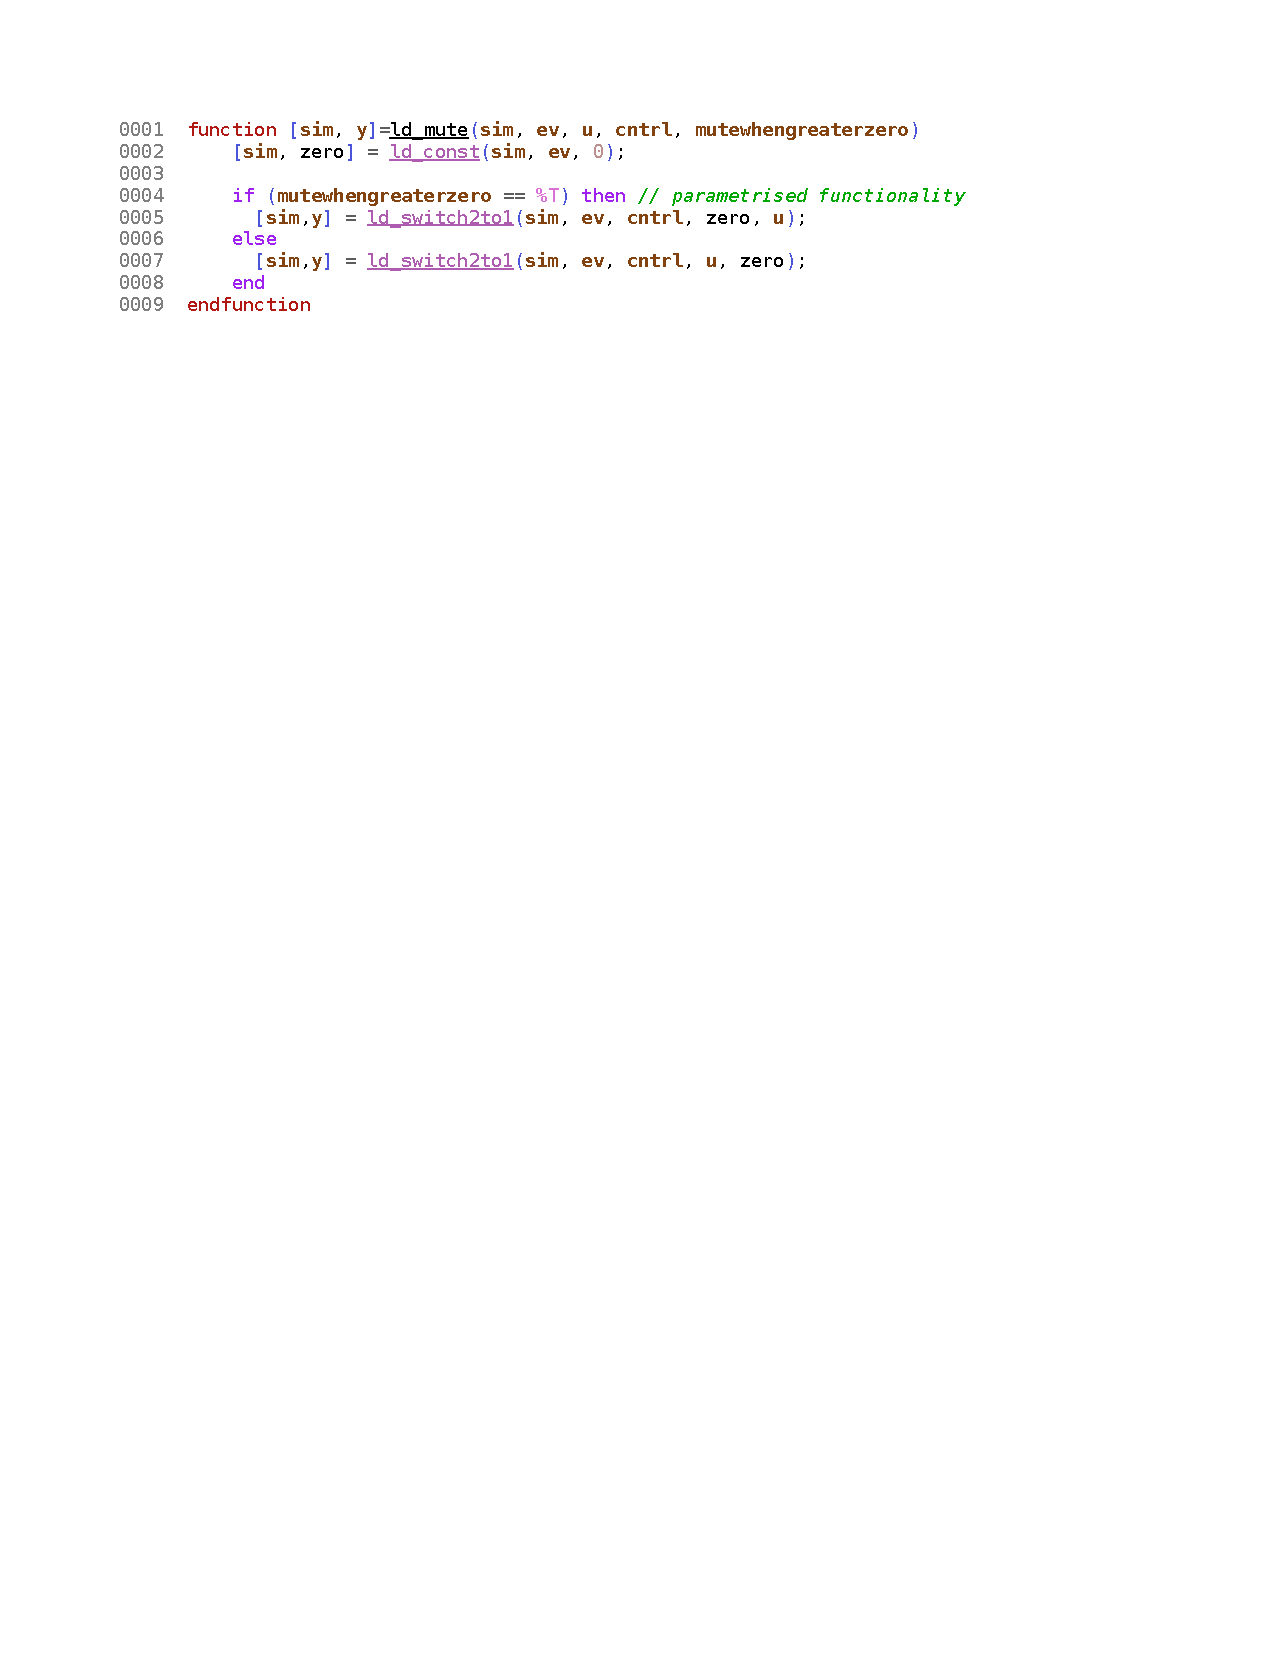
\includegraphics[trim=3cm 22cm 4cm 1.4cm, clip, width=0.85\linewidth]{figures/ld_mute.pdf} 


% {\small 
% \begin{lstlisting} 
% function [sim, y] = ld_mute( sim, ev, u, cntrl, mutewhengreaterzero )
%     [sim, zero] = ld_const(sim, ev, 0);
%     
%     if (mutewhengreaterzero == %T) then
%       [sim,y] = ld_switch2to1(sim, ev, cntrl, zero, u);
%     else
%       [sim,y] = ld_switch2to1(sim, ev, cntrl, u, zero);
%     end
% endfunction
% \end{lstlisting}
% }

\begin{itemize}
 \item This example describes a superblock, which has two inputs \texttt{u} and \texttt{cntrl} and one output \texttt{y}.
\item \texttt{mutewhengreaterzero} describes a parameter.
\item \textbf{NOTE}: With the if / else construction a superblock can have different behaviour depending on a parameter! (This enables great possibilities for creating reusable code)
\end{itemize}


\end{frame}


\begin{frame}[fragile]
 \frametitle{Superblocks: Usage}
 
%  \begin{itemize}
  Once defined, the superblock can be used like any other ORTD-Block:
%  \end{itemize}

\vspace{1.5cm}
 
 {\small 
\begin{lstlisting} 
 [sim, y] = ld_mute( sim, ev, u=input, cntrl=csig, ...
                     mutewhengreaterzero=%T ) 
\end{lstlisting}}

\end{frame}




\begin{frame}[fragile]
 \frametitle{Feedback Loops}

\textbf{How to implement feedback?}

  \begin{itemize}
   \item A dummy signal is required, which can be used to connect a real block:
  \end{itemize}
% To initialise a signal, which comes from an (at the current definition step) unknown source \texttt{libdyn\_new\_feedback} is used:

  {\small 
  \begin{lstlisting} 
  [sim, feedback] = libdyn_new_feedback(sim);
  \end{lstlisting}}

  \begin{itemize}
%    \item Now, the signal \texttt{feedback} can be used like an usual signal.
   \item Later in the ongoing code, the loop is closed via \texttt{libdyn\_close\_loop}, which means \texttt{feedback} is assigned to a real signal \texttt{y}:
  \end{itemize}

  {\small 
  \begin{lstlisting} 
  [sim] = libdyn_close_loop(sim, y, feedback);
  \end{lstlisting}}
  
\end{frame}





\begin{frame}[fragile]
 \frametitle{Feedback Loops: An example}



\centering 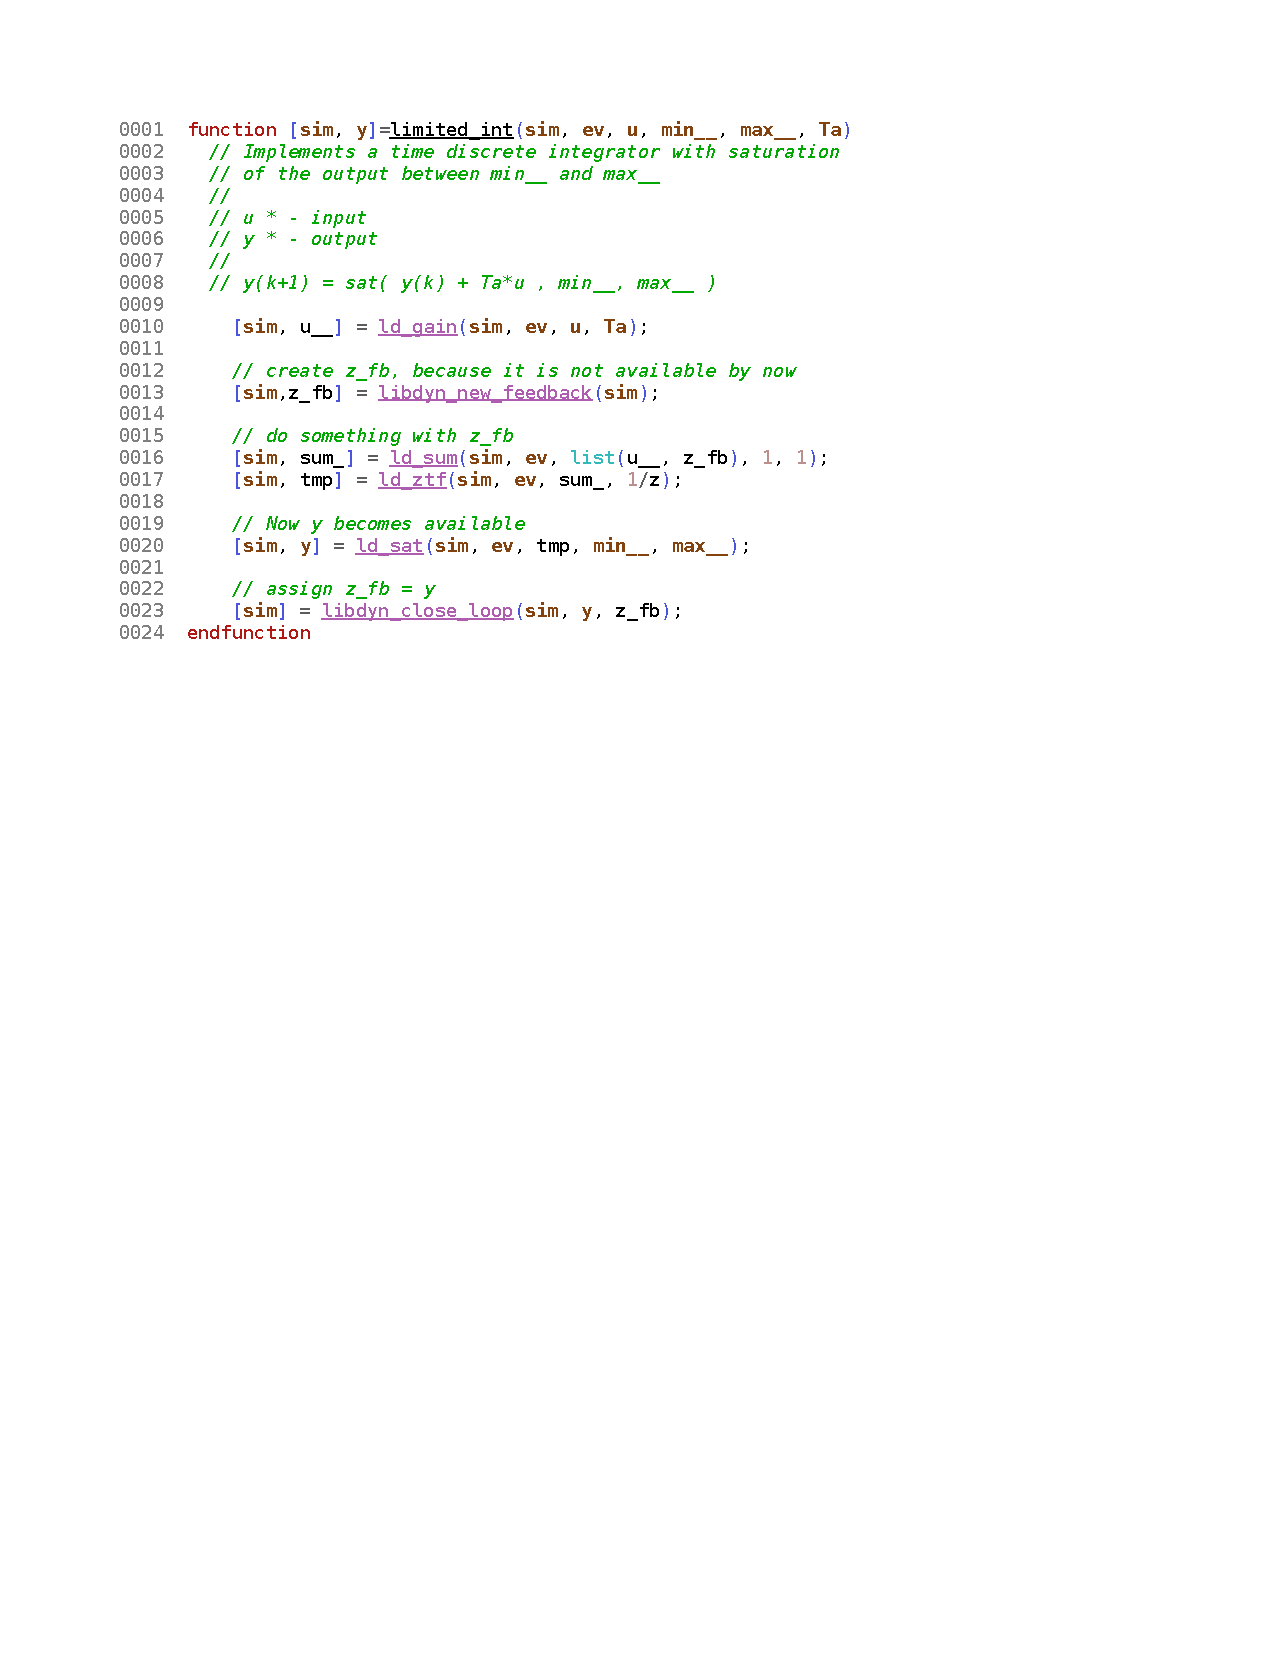
\includegraphics[trim=3cm 16.5cm 4cm 1cm, clip, width=0.8\linewidth]{figures/limited_int.pdf} 

\centering 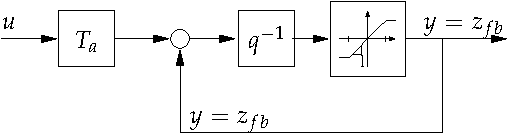
\includegraphics[width=0.6\linewidth]{figures/ld_limited_int_block.pdf} 


\end{frame}





\begin{frame}[fragile]
 \frametitle{Example: Lookup table for multiple channels}




  \mbox{

\hspace{-1cm}

     \begin{minipage}{0.7\linewidth}
       \vspace{-0.5cm}
	\centering 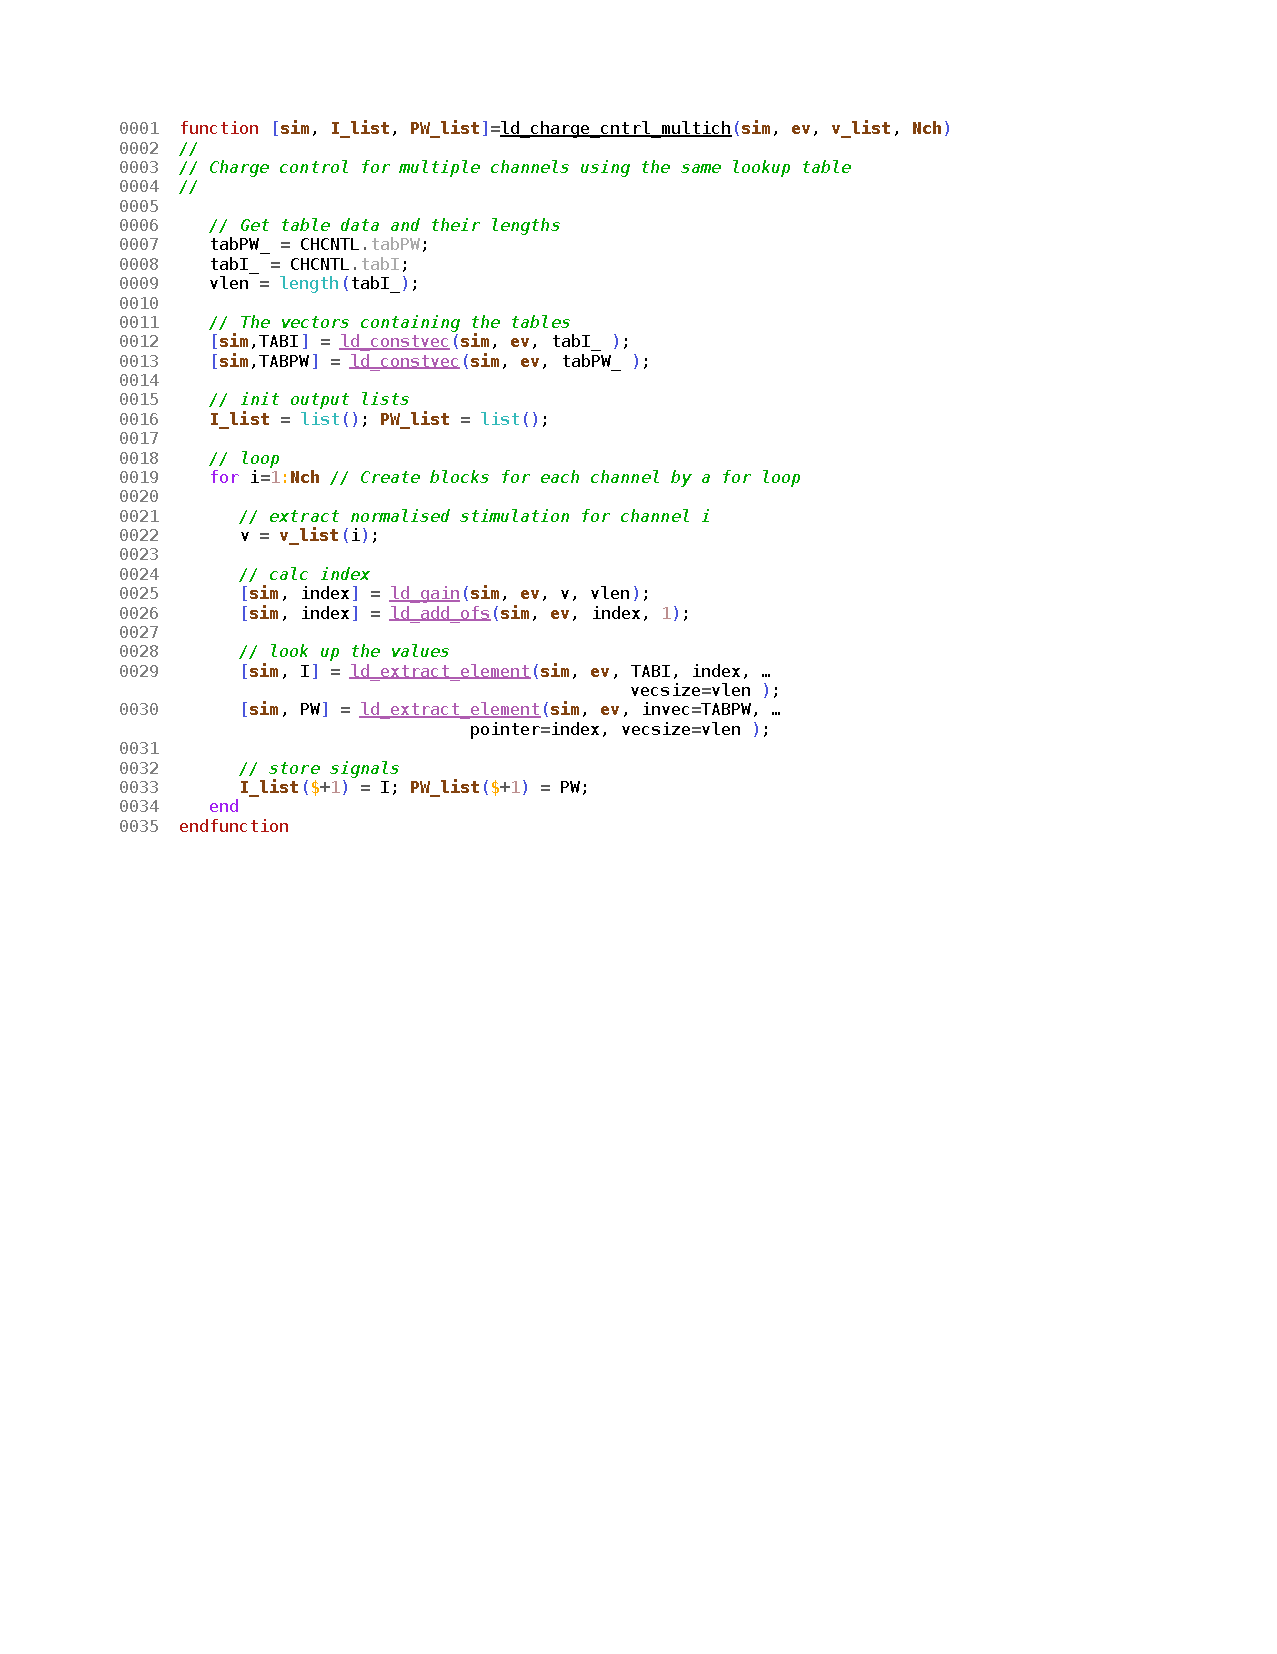
\includegraphics[trim=3cm 9.5cm 4cm 1cm, clip, width=1.3\linewidth]{figures/ld_charge_cntrl_multich.pdf} 

     \end{minipage}

     \begin{minipage}{0.55\linewidth}
\hspace{-1.8cm}
\vspace{2cm}
	\centering 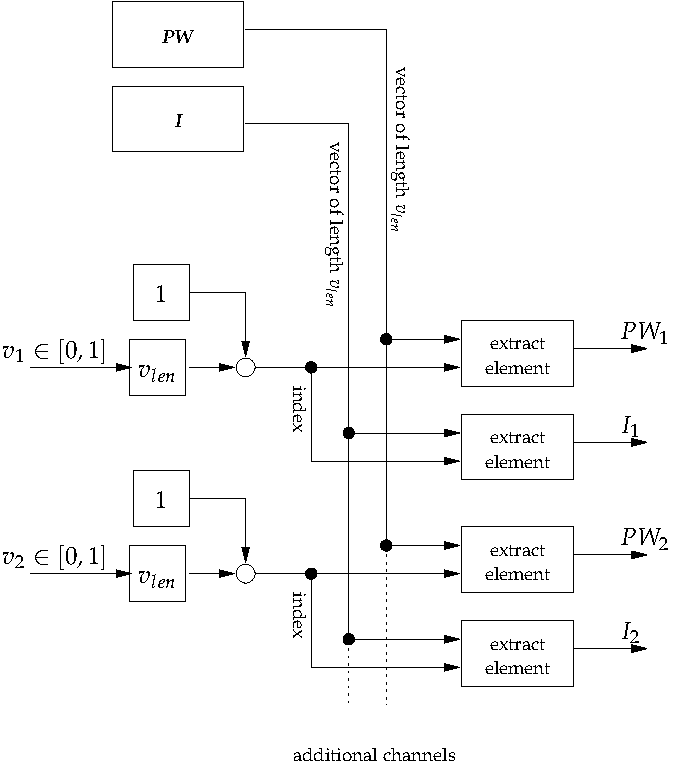
\includegraphics[width=1.0\linewidth]{figures/charge_control.pdf} 

     \end{minipage}    
  }

\end{frame}



\begin{frame}
  \frametitle{State machines}

  \textbf{Principle:}

  \begin{itemize}
   \item Each state is represented by a one sub-schematic. 
   \item Indicating the current state, only one schematic is active at once. State related computations are performed while the state is active.
   \item The active sub-schematic may cause the transition to another state at any time.
  \end{itemize}

  \textbf{Extra features:}
  \begin{itemize}
   \item When a state is left, the corresponding schematic is reset.
   \item Possibility to share variables among states; to e.g. realise counters, ...
  \end{itemize}

  
  

\end{frame}

\begin{frame}
  \frametitle{State machines: implementation}

% \begin{itemize}
%  \item 
One superblock-function is evaluate for each state. Differentiation among states may be realised by using a \texttt{select} statement:
% \end{itemize}
  

\centering 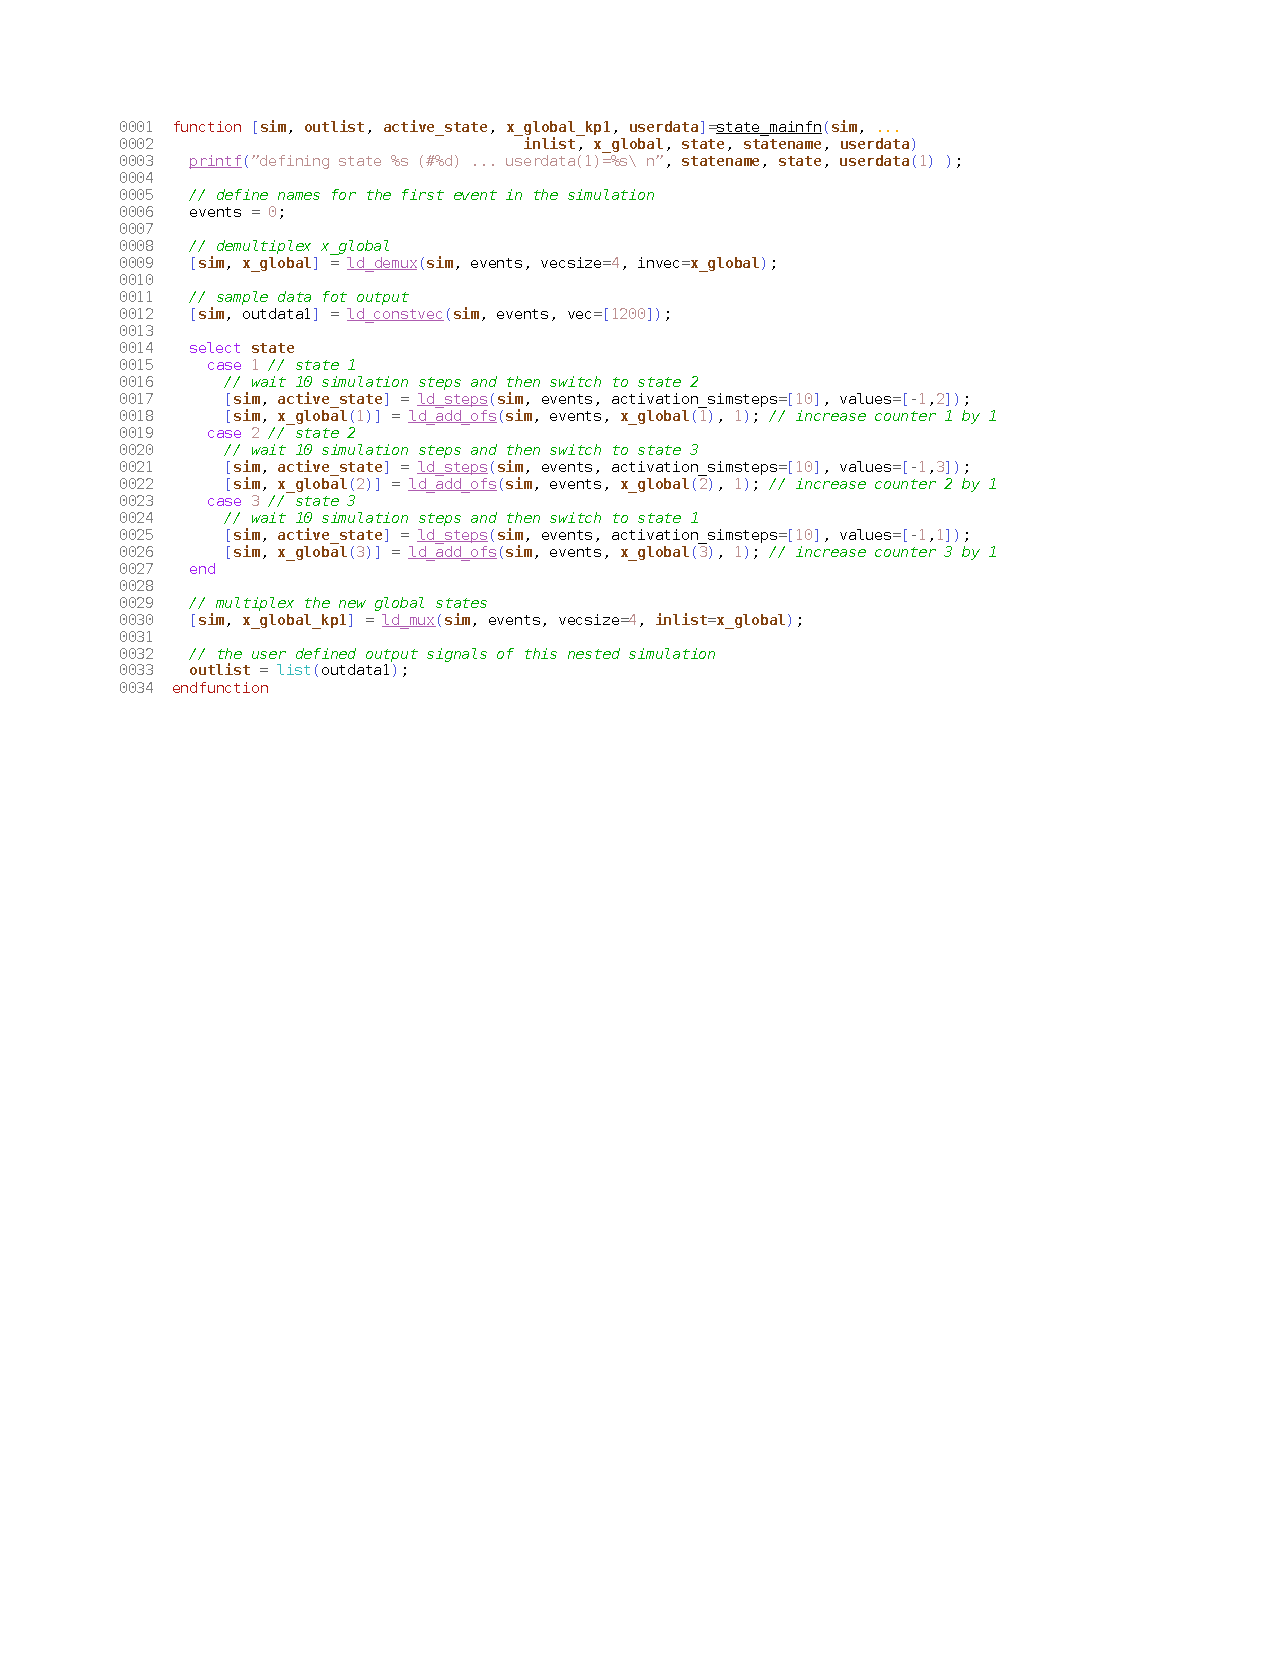
\includegraphics[trim=2.7cm 9.5cm 4cm 1.4cm, clip, width=1.0\linewidth]{figures/state_mainfn.pdf} 

\end{frame}


\begin{frame}
  \frametitle{Threads}

  \centering 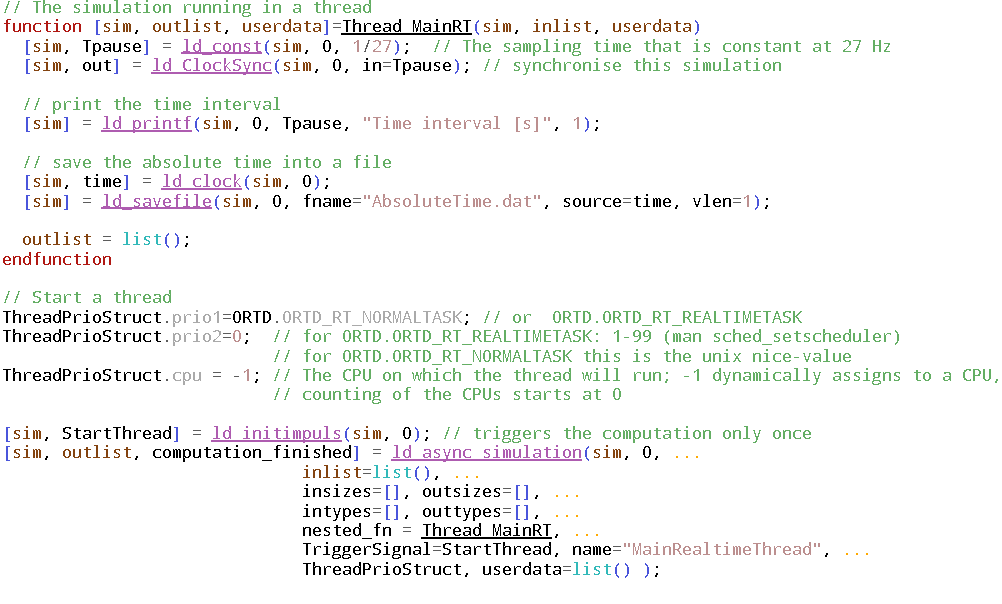
\includegraphics[width=1\linewidth]{figures/Threads_crop.pdf} 
\end{frame}

\begin{frame}
  \frametitle{Remote Control Interface -- I}

  \begin{itemize}
    \item Send and receive data/streams via packet-based communication channels, e.g. UDP
  \end{itemize}
  \centering 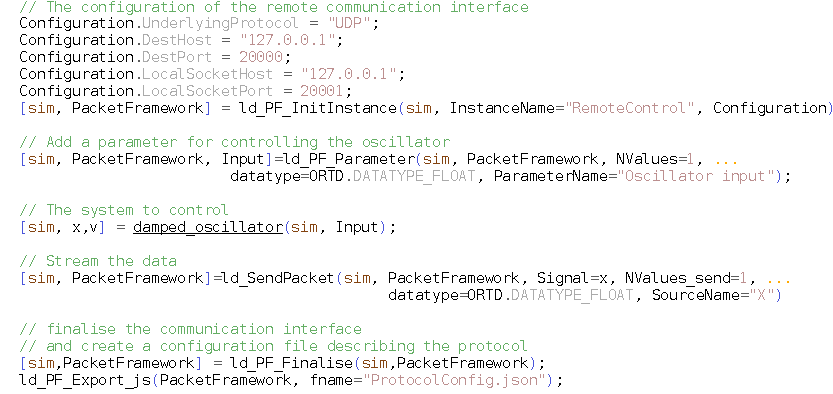
\includegraphics[width=1\linewidth]{figures/RemoteControl_Cut_crop.pdf} 

\end{frame}

\begin{frame}
  \frametitle{Remote Control Interface -- II}

  \begin{itemize}
    \item Use e.g. a node.js program to build a web-interface to visualise data and to edit parameters.
  \end{itemize}

  \centering 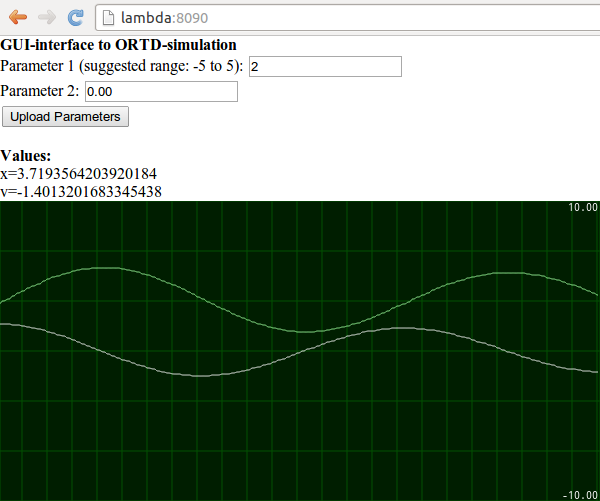
\includegraphics[width=0.8\linewidth]{figures/Webinterface.png} 

\end{frame}


\begin{frame}
  \frametitle{Automatic calibration procedures}
  \begin{itemize}
    \item Allows to easily implement automated calibration procedures. The calib. routine may also be implemented using normal Scilab code.
  \end{itemize}
  \centering 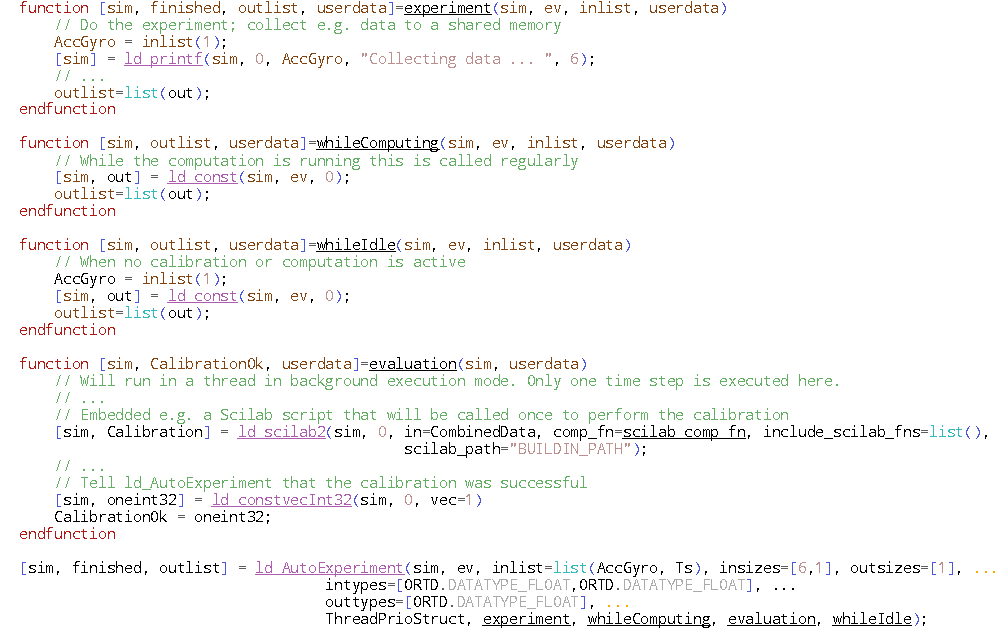
\includegraphics[width=1\linewidth]{figures/Autocalibration_crop.pdf} 

\end{frame}



\begin{frame}
Examples for advanced features like 

  \begin{itemize}
\item Online replacement of sub-controllers (\texttt{modules/nested})
\item State machines (\texttt{modules/nested})
\item Simulations running in threads (\texttt{modules/nested})
\item Shared memory, circular buffers, sending events to threads, ...
\item Mathematical formula parsing (\texttt{modules/muparser})
\item Vector/matrix operations (\texttt{modules/basic\_ldblocks})
\item Embeding Scilab-code (\texttt{modules/scilab})
\item Starting, I/O to external processes (\texttt{modules/ext\_process})
\item Variable sampling rates (\texttt{modules/synchronisation})
\item Scicos to ORTD block wrapper (\texttt{modules/scicos\_blocks})
\item UDP-communication \& remote control interface (\texttt{modules/udp\_communication})
\item ...
  \end{itemize}

  can be found within the directories \texttt{modules/*/demo}. Most of them are ready to run.
\end{frame}




\end{document}
